%
% Credit to Tibault Reveyrand for the initial template - https://www.overleaf.com/articles/ieee-journal-submission-trans-on-mtt-example/pbfcbcjvmvmn

% ================================================
% Please HIGHLIGHT the new inputs such like this :
% Text :
%  \hl{comment}
% Aligned Eq. 
% \begin{shaded}
% \end{shaded}
% ================================================


\documentclass[journal]{IEEEtran}

%\usepackage[retainorgcmds]{IEEEtrantools}
%\usepackage{bibentry}  
\usepackage{xcolor,soul,framed} %,caption

\colorlet{shadecolor}{yellow}
% \usepackage{color,soul}
\usepackage[pdftex]{graphicx}
\graphicspath{{../images/}}
\DeclareGraphicsExtensions{.pdf,.jpeg,.png}

\usepackage[cmex10]{amsmath}
%Mathabx do not work on ScribTex => Removed
%\usepackage{mathabx}
\usepackage{array}
\usepackage{mdwmath}
\usepackage{mdwtab}
\usepackage{eqparbox}
\usepackage{url}

\hyphenation{op-tical net-works semi-conduc-tor}

%\bstctlcite{IEEE:BSTcontrol}


%=== TITLE & AUTHORS ====================================================================
\begin{document}
\bstctlcite{IEEEexample:BSTcontrol}
    \title{Screening  Radiology  Images  for Lesion  Detection: An ML Approach}
  \author{Teodor~Ilie,~Jihyeon~Park,~and~Alex~Sun% <-this % stops a space

}  

% The paper headers
\markboth{}{}

% ====================================================================
\maketitle


% === 1. ABSTRACT ====================================================================
% =================================================================================
\begin{abstract}
%\boldmath
Radiologists manually evaluate large volumes of CT scans daily, and with this large workload comes the possibility of human error. Recent years have seen a rise in ``reckless-reading lawsuits", accusing radiologists of spending insufficient time viewing images, and leading to missed findings. At the same time, it is not unusual for experts to view images for only a second, and there is no clear research indicating that enforcing longer viewing times would improve accuracy; rather the issue is often with human error brought on by fatigue. \cite{workload}

To improve the interpretation process, we propose employing AI models to give radiologists an additional tool to assist with their analysis, particularly for identifying lesions. Using the massive DeepLesion \cite{deeplesion} dataset, we train and test a range of state-of-the-art models to generate bounding boxes for lesions, given CT scans as input, and determine which produces the most accurate results. 

\hl{Discuss results here when available.}

The output of our model can be deployed for use in hospitals, and be further inspected by radiologists to determine malignancy and subsequent treatment. We argue that such a tool improves the performance of human analysis alone, mitigating human error caused by fatigue, long hours, and other challenging circumstances radiologists face. \end{abstract}

\begin{IEEEkeywords}
Radiology, DeepLesion, Convolutional Neural Network, U-Net, YOLO
\end{IEEEkeywords}


% === II. BACKGROUND =============================================================
% =================================================================================
\section{Background}
\subsection{CT Scans and Radiologist Workload}
% =======
% FIG. 01
% =======
% \begin{figure}
%  \begin{center}
%  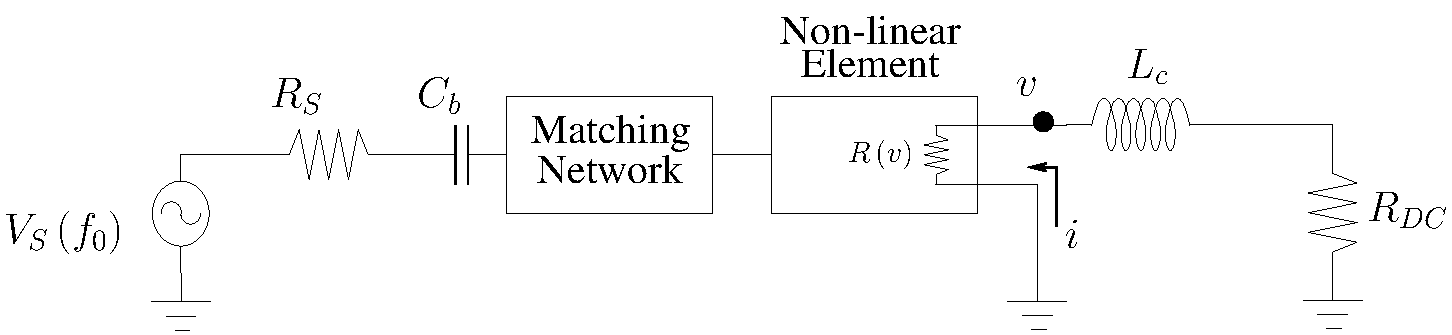
\includegraphics[width=3.5in]{pdf/01.pdf}\\
%  \caption{Caption}\label{circuit_diagram}
%  \end{center}
%\end{figure}

\IEEEPARstart{C}{omputed} Tomography (CT) scanners take many cross-sectional areas at fixed-length intervals along a specific body part, generating dozens or even hundreds of scans depending on the area of interest \cite{PMID:33620865}. There are many use cases for CT scans including preventative medicine and cancer screening, but scanning for lesions is particularly useful. A lesion is visible on a CT scan as it looks abnormal from the surrounding tissue, and radiologists manually inspect scans to determine parameters like the size and shape of the lesion. Lesions fall into several categories, including benign lesions such as cysts and fibromas, cancerous lesions such as tumours and metastases, and infectious lesions such as abscesses and granulomas. Lesion types cannot always be classified from CT scans alone, and subsequent tests such as biopsies, additional imaging tests such as MRI and ultrasound, blood tests, and others are used to determine the lesions cause and treatment courses \cite{oncology}.

% =======
% FIG. 01
% =======
\begin{figure}
 \begin{center}
 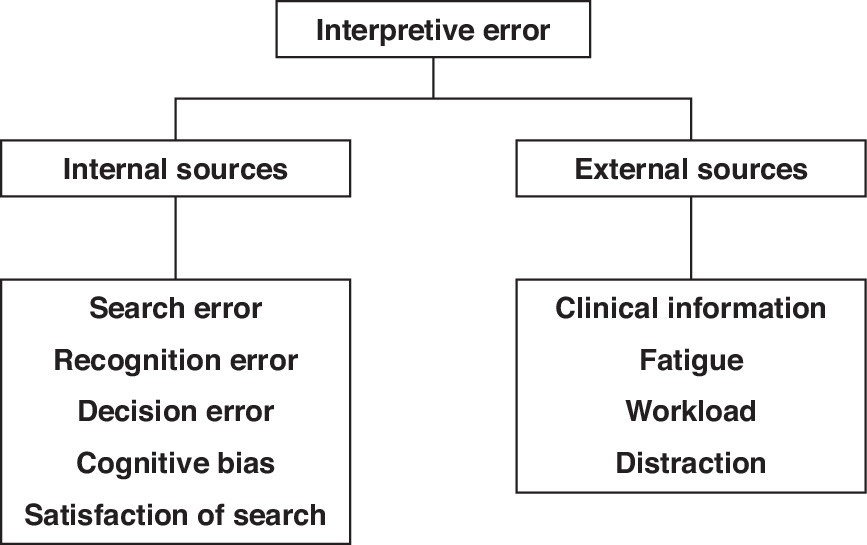
\includegraphics[width=3.5in]{images/scan_error.jpeg}\\
 \caption{Categories of interpretive error, both internal and external \cite{radiology_error}.}\label{interpret_error}
 \end{center}
\end{figure}

As the use of medical imaging such as CT scans continues to grow due to its numerous applications, radiologists are in increasing demand, yet expert radiologists are a scarce resource due to the time and challenges of training. This is placing increasing strain on the time and resources of existing radiologists, leading to climbing medical errors brought on by fatigue, and it is a leading cause of litigation. Medical error is a serious issue; Makary et al. have argued that should medical error, in general, be treated as a disease, it would rank as the third top cause of death in the US \cite{medical_error}. 

An overview of the most common ways radiologists are affected by interpretive error is given in Figure \ref{interpret_error}. Funaki et al. have determined that as much as 60-80\% of errors, depending on the context, are caused by perception error \cite{perception_error}. In addition, there has been a sevenfold increase in image interpretations performed per minute from 1999 to 2000, which is likely causing human errors to increase due to fatigue from the increased workload \cite{radiology_error}. 

At the same time, it is challenging to determine and implement meaningful workload limitations for radiologists, given the complexity of the process and the variation from person to person. While it is well-established that reducing the viewing time negatively affects interpretation accuracy, prescribing blanket variations for all radiologists would also be arbitrary and ineffective, as such regulations would not account for the varying degrees to which different people are affected by the same circumstances. As such, radiologists continue to self-regulate the workload to a great extent. Furthermore, external factors such as distraction and cognitive biases are even more challenging to address with regulation or training \cite{workload}. 

\subsection{Improvements through AI}
Many of these human errors have the potential to be dramatically improved through the use of computer-aided diagnosis, and in particular, modern AI image recognition models. With lesion detection being one of the most important yet time-consuming tasks of radiologists, such a tool would be immensely useful \cite{deep_learning_survey}. As these models continue to improve, they have already seen successful applications in providing radiologists with a second opinion in real-time, acting as a ``safety net". Of particular interest is the fact that they are entirely unaffected by human errors of bias and fatigue, and as algorithms continue to improve, their perceptual abilities begin to compete with that of even trained radiologists \cite{workload}. Some experts even go so far as to claim that radiologists will gradually be altogether replaced by better-performing, cheaper, and faster AI systems \cite{ai_foe}, while others maintain that radiologists will continue to play the central role, and AI tools will remain just that - an additional tool to enhance their work quality \cite{doctors_ftw}. Either way, the consensus is clearly in favour of the benefits of increasing the quality and roll-out of AI models for improved diagnostic accuracy and quality, and its potential to save lives \cite{consensus}\cite{ai_adoption}. 

\hl{Explain basic function and performance of CNNs, Faster R-CNN, U-NET, and other models we decide to use.}


% === III. HYPOTHESIS ========================
% =================================================================================
\section{Hypothesis}
Our primary aim is to explore the accuracy with which an AI model can generate bounding boxes for lesions on CT scan images, as compared to the ground truth. We hypothesize that state-of-the-art image recognition algorithms are able to perform on-par, or even exceed, expert analysis.

% === IV. METHODS ========================
% =================================================================================
\section{Methods}
We train our model on the DeepLesion dataset, which contains 32,735 lesions in 32,120 CT slices from 10,594 studies of 4,427 unique patients \cite{deeplesion}. This dataset is publicly available and does not require special access permissions. The data is gathered from CT scan images that were annotated by radiologists during routine analysis, and stored as ``bookmarks" in hospitals' picture archiving and communication systems (PACS).  

Every image is annotated with a bounding box surrounding lesions, and each lesion contains information about the lesion diameter and lesion type.
We will compare various models such as CNN (Convolutional Neural Networks), U-Net (a type of CNN architecture well-suited for semantic segmentation), and Faster R-CNN (a faster version of R-CNN that searches for objects using region proposals) \hl{This may be addressed in background, and should be adjusted based on the models we end up choosing}. We will determine the speed and accuracy trade-offs of these models, using the Dice-Sørensen coefficient to compare our model’s performance relative to the original bounding boxes.

To ensure that the data is not skewed, we will ensure the data is split by patient into training, validation and testing. By splitting the data, we can check the performance of our model on new data that was not used for training \cite{chollet_deep_learning}. We will also attempt to address the possibility of skewed data due to all images in the dataset containing a lesion, and some lesions not being annotated \cite{deeplesion}. The proposed fix is to remove lesions for part of the data somehow, either by slicing out part of the image entirely or by using content-aware filling, such that our model will not be biased towards always predicting lesions on scans.

\hl{Discuss data pre-processing here, once we have results.}

% === V. RESULTS ========================
% =================================================================================
\section{Results}
\hl{TBD}

% === VI. DISCUSSION ========================
% =================================================================================
\section{Discussion}
\hl{Based on results, discuss how close we came to the ground truth in the original DeepLesion annotations. Discuss that there is bias due to the lack of images with no lesions. Discuss that there are some lesions not annotated as the radiologists were not interested in fully annotating the images, as they were not explicitly meant for training a DL model.

Discuss possible use cases, how similar models have been deployed in practice up to now, and how such models have performed.}

\section*{Team Reflection}
All three of the authors have a background in computer science, and not biology. As such, our focus was on processing the data and implementing AI models with high accuracy, and not on the underlying biological significance of lesions.

\bibliographystyle{IEEEtran}
\bibliography{IEEEabrv,Bibliography}

\vfill
\end{document}

% An example of a floating figure using the graphicx package.
% Note that \label must occur AFTER (or within) \caption.
% For figures, \caption should occur after the \includegraphics.
% Note that IEEEtran v1.7 and later has special internal code that
% is designed to preserve the operation of \label within \caption
% even when the captionsoff option is in effect. However, because
% of issues like this, it may be the safest practice to put all your
% \label just after \caption rather than within \caption{}.
%
% Reminder: the "draftcls" or "draftclsnofoot", not "draft", class
% option should be used if it is desired that the figures are to be
% displayed while in draft mode.
%
%\begin{figure}[!t]
%\centering
%\includegraphics[width=2.5in]{myfigure}
% where an .eps filename suffix will be assumed under latex, 
% and a .pdf suffix will be assumed for pdflatex; or what has been declared
% via \DeclareGraphicsExtensions.
%\caption{Simulation Results}
%\label{fig_sim}
%\end{figure}

% Note that IEEE typically puts floats only at the top, even when this
% results in a large percentage of a column being occupied by floats.


% An example of a double column floating figure using two subfigures.
% (The subfig.sty package must be loaded for this to work.)
% The subfigure \label commands are set within each subfloat command, the
% \label for the overall figure must come after \caption.
% \hfil must be used as a separator to get equal spacing.
% The subfigure.sty package works much the same way, except \subfigure is
% used instead of \subfloat.
%
%\begin{figure*}[!t]
%\centerline{\subfloat[Case I]\includegraphics[width=2.5in]{subfigcase1}%
%\label{fig_first_case}}
%\hfil
%\subfloat[Case II]{\includegraphics[width=2.5in]{subfigcase2}%
%\label{fig_second_case}}}
%\caption{Simulation results}
%\label{fig_sim}
%\end{figure*}
%
% Note that often IEEE papers with subfigures do not employ subfigure
% captions (using the optional argument to \subfloat), but instead will
% reference/describe all of them (a), (b), etc., within the main caption.


% An example of a floating table. Note that, for IEEE style tables, the 
% \caption command should come BEFORE the table. Table text will default to
% \footnotesize as IEEE normally uses this smaller font for tables.
% The \label must come after \caption as always.
%
%\begin{table}[!t]
%% increase table row spacing, adjust to taste
%\renewcommand{\arraystretch}{1.3}
% if using array.sty, it might be a good idea to tweak the value of
% \extrarowheight as needed to properly center the text within the cells
%\caption{An Example of a Table}
%\label{table_example}
%\centering
%% Some packages, such as MDW tools, offer better commands for making tables
%% than the plain LaTeX2e tabular which is used here.
%\begin{tabular}{|c||c|}
%\hline
%One & Two\\
%\hline
%Three & Four\\
%\hline
%\end{tabular}
%\end{table}


% Note that IEEE does not put floats in the very first column - or typically
% anywhere on the first page for that matter. Also, in-text middle ("here")
% positioning is not used. Most IEEE journals use top floats exclusively.
% Note that, LaTeX2e, unlike IEEE journals, places footnotes above bottom
% floats. This can be corrected via the \fnbelowfloat command of the
% stfloats package.


